\graphicspath{{./ch_theory_and_methods/figures/}}


\chapter{Experimental control and theory of the NV center}
\label{ch:TAM}

\begin{center} 
    \vspace{-1cm} {M.S.~Blok} 
\end{center}


\vspace{-0.5cm} 
The Nitrogen-Vacancy (NV) center in diamond has recently emerged as an excellent system to demonstrate quantum control of single spins. In this chapter we discuss its physical properties and the experimental techniques that form the basis of the results presented in chapters \ref{ch:AMC}-\ref{ch:CDL}. We first introduce the basic electronic structure and the detection of single NV centers in a confocal microscope setup (section \ref{sec:NVcenter}). In section \ref{sec:devices} we discuss the devices that enable optical initialization and single shot readout of the electron spin at low temperature (section \ref{sec:opticalcontrol}). The coherent control and characterization of the coherence times of the electron spin are presented in section \ref{sec:groundstatecontrol}. Finally we show how the coupling of the central spin to nearby nuclear spins allows us to extend our quantum register to multiple qubits.
\clearpage


\section{The NV center in diamond}
\label{sec:NVcenter}

The nitrogen vacancy center is a defect in the diamond lattice consisting of a substitutional nitrogen atom and a vacancy at an adjacent lattice position (Fig. \ref{fig:tam-fig1-nvstruct}). In its neutral charge state ($NV^{0}$) it hosts 5 electrons: 2 donor electrons from the nitrogen and 3 from the dangling bonds of the adjacent carbon atoms. Its negative charge state $NV^{-}$ is formed by capturing an electron from the environment. The experiments in this thesis are all performed on $NV^{-}$, which can be prepared experimentally as discussed in section \ref{sec:opticalcontrol}.

\begin{figure*}
	\centering
	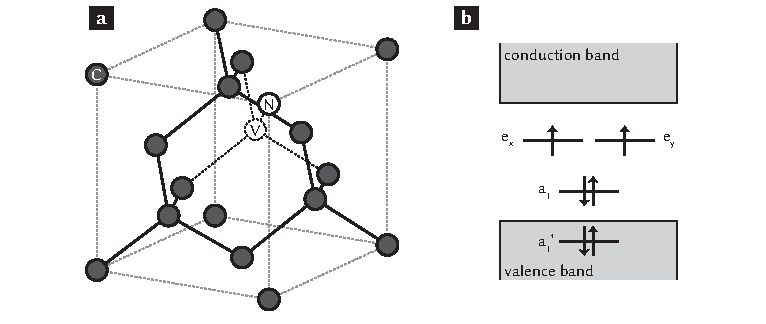
\includegraphics{figure_NV-structure-bernien}
	\caption{\label{fig:tam-fig1-nvstruct} \textbf{Crystal and electronic structure of the NV center} Figure from \cite{Bernien__2014}(a) The Nitrogen-Vacancy center defect is formed by a substitutional nitrogen atom (N) and a missing atom (vacancy, V) at an adjacant position in the diamond lattice (b) The electron occupation of the molecular orbitals in the electronic ground state, following Pauli's exclusion principle. The molecular orbitals are a linear combination of hybridised $sp^3$-orbitals. They are found by using the $C_{3v}$-symmetry of the NV center, taking into account the Coulomb interaction of the diamond nuclei and the lattice electrons with the electrons in the orbitals.}
\end{figure*}

In the electronic ground state, the 6 electrons occupy the molecular orbitals as shown in Fig. \ref{fig:tam-fig1-nvstruct}b. Excluding electron-electron interactions, the electronic ground-, ($^2a^2e$) and excited ($^1a^3e$) state are spin degenerate. This degeneracy is lifted by the Coulomb interaction between the electrons which leads to spin triplet (S = 1) ground-, and excited states ($^3A_2$ and $^3E$ respectively) as well as multiple intermediate spin singlet levels. The $^3A_2$ to $^3E$ transition energy of 1.945 eV lies in the optical regime (637 nm), well within the bandgap of diamond (5.5eV). Since all experimental techniques in this thesis aim to control the NV center in the spin triplet manifold, we will not discuss the singlet levels in further detail. For a more detailed discussion of the electronic structure of the NV-center we refer to a recent review of Doherty \textit{et al} \cite{Doherty_PhysicsReports_2013}.

\begin{figure*}
	\centering
	\includegraphics{figure_single_NVs-bernien}
	\caption{\label{fig:tam-fig2-nvstruct} \textbf{Detection of single NV centers} Figure from \cite{Bernien__2014}(a) Confocal microscope setup. The NV centers are excited by focussing a green (532 nm) excitation laser onto the sample using a microscope objective (MO). The sample is mounted on a piezo-stage allowing three-dimensional scans. The emission is spectrally filtered using a dicroic mirror (DM) and via a mechanically switchable mirror (FM) sent either to a spectrometer or to a beamsplitter (BS) followed by two APDs in a HBT-configuration. (b) Confocal scan of a bulk diamond sample. The intensity is plotted as a function of the stage position in \textit{x} and \textit{y}. Blue is higher intensity. (c) Emission spectrum of a single NV center with the zero phonon line at 637 nm and the phonon sideband at higher wavelengths. (d) Second-order autocorrelation function, with $\tau$ the delay between detection events of different detectors. The solid-line is a fit using a three-level model, including dark counts. The slow decay is associated with the decay from the singlet levels.}
\end{figure*}

We identify NV centers in bulk diamond at room-temperature in a home-build confocal microscope setup (Fig. \ref{fig:tam-fig2-nvstruct}a). By scanning the sample and collecting the fluorescence signal with a single photodiode (APD) we find multiple diffraction limited spots, corresponding to NV centers (Fig. \ref{fig:tam-fig2-nvstruct}b). Here we off-resonantly excite the NV center to a phonon level above the $^3E$ level, which quickly decays non-radiatively to $^3E$. The reflections of the excitation are separated from the fluorescence with a dicroic mirror. The emission spectrum from $^3E$ is show in Fig. \ref{fig:tam-fig2-nvstruct}c. It shows a distinct peak around 637 nm, corresponding to the direct decay from $^3E$ to $^3A_2$ (zero phonon line, ZPL) and a broad sideband corresponding to the decay to a phonon level above $^3A_2$ (phonon side band, PSB). To verify that the signal originates from a single emitter, we measure the second-order autocorrelation function $g^2 (\tau)$ in a Hanbury-Brown-Twiss configuration (Fig. \ref{fig:tam-fig2-nvstruct}d). The low probability of simultaneous photon detection ($g^2 (\tau = 0) < 1/2$) confirms that the signal comes from a single emitter.

\section{Single NV center device}

To enhance the collection and excitation efficiency of the NV center, a solid-immersion lens (SIL) is milled in the diamond using a focused ion beam (FIB) \cite{Hadden__2010,Marseglia__2011,Bernien__2014,Jamali__2014} (Fig. \ref{fig:tam-fig3-device}a). For an NV center in the middle of the SIL, the hemisphere ensures that the emission from the NV center reaches the diamond-air surface at normal incidence. This significantly reduces the loss due to total-internal reflection. For precise placement of the SIL, a pre-characterized NV center is located with respect to 1x1 $\mu$m gold markers that are fabricated on the surface of the diamond using electron beam lithography. The hemisphere structure is then created using a gallium ion beam by milling concentric rings of varying diameter around the position of the NV center. After milling the SILs, the sample is cleaned for 30 minutes in a boiling mixture of equal parts of perchloric, sulforic and nitric acid. This step removes the redeposited material during milling. A small conductive layer of gallium atoms that is implanted during the FIB process is removed by reactive-ion etching in an oxygen-plasma. 
\label{sec:devices}
\begin{figure*}
	\centering
	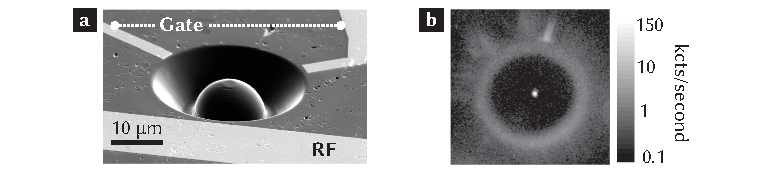
\includegraphics{figure_SIL_finished-bernien}
	\caption{\label{fig:tam-fig3-device} \textbf{} Figure from \cite{Bernien__2014} (a) }
\end{figure*}

A 200 nm thick gold microwave strip line for spin manipulation (Fig \ref{fig:tam-fig7-erabi} and \ref{fig:tam-fig10-nrabi}) and DC gates to DC stark shift the ZPL (see chapter \ref{ch:LDE}) are  fabricated near the SIL using electron beam lithography. Finally a single-layer anti-reflection coating\cite{Yeung__2012} (aluminium oxide) is fabricated on top of the sample to further increase the collection efficiency and reduce the reflection during resonant excitation (see chapter \ref{ch:LDE}).

\section{Addressing the electron excited state}
\label{sec:opticalcontrol}

The spin-orbit and spin-spin interactions introduce a fine splitting to the $^3E$ excited state which can be observed at cryogenic temperatures. The six resulting transitions have a distinct spin character (Fig. \ref{fig:tam-fig4-laserscan}a) and allow for spin-selective optical excitation of the electron. The transitions to the $m_s = 0$ states ($E_x$ and $E_y$) can occur upon absoprtion or emission of a linearly polarized photon, while the four $m_s = \pm 1$ transitions couple to circularly polarized light. The transition frequencies shift when an electric field or strain is applied. For an electric field along the N-V axis this results in an offset to the spectrum, not changing the energy level spacing. A perpendicular electric field affects the difference between the energy levels. As a result, the spectrum of the excited state slightly varies between NV centers due to local differences in strain and electric field. In Fig. \ref{fig:tam-fig4-laserscan}b we show measurements of the spectra of three different NV centres, normalized to have the same parallel strain. The lateral strain is determined from the difference between the transition energies of $E_x$ and $E_y$. The spectra show excellent agreement with the theoretical prediction (dashed lines). The strain typically differs a few tens of GHz between NV centers measured in this thesis.

\begin{figure*}
	\centering
	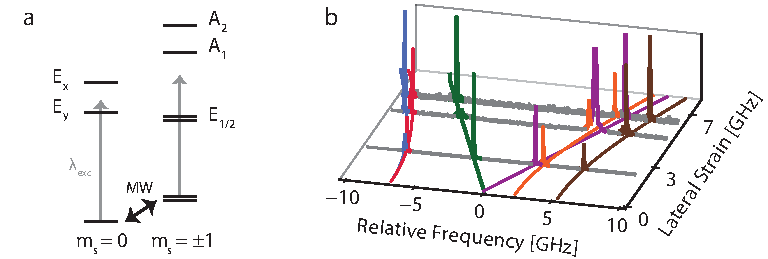
\includegraphics{laserscans}
	\caption{\label{fig:tam-fig4-laserscan} \textbf{Spectrum of the excited state} (a) Energy level diagram of the fine structure of the excited states. There are two levels with spin $m_s = 0$ ($E_x$,$E_y$) and four $m_s = \pm 1$ levels ($A_1$,$A_2$,$E_1$ and $E_2$). At finite strain the degeneracies between $E_x$,$E_y$ and $E_1$,$E_2$ are lifted. (b) The energy spectrum for three different NV centers is measured by varying the frequency of the excitation laser and detecting the fluorescence in the PSB. The observed transitions $E_1$ (blue), $E_2$ (red), $E_y$ (green), $E_x$ (purple), $A_1$ (orange) and $A_2$ (brown) are color coded and agree well with the theoretical prediction (colored dashed lines). For each scan the transition energies $\Delta E_x$ and $\Delta E_y$ are determined to calculate the lateral ($\frac{\Delta E_x-\Delta E_y}{2}$) and parallel ($\frac{\Delta E_y+\Delta E_x}{2}$) strain. The parallel strain is then substracted for each scan. Laser frequency is with respect to 470.4 THz.}
\end{figure*}

To address the spin-selective optical transitions in an experiment, we first verify that the NV center is in the $NV^-$ state and that the lasers are resonant with the desired transitions before each experimental run. During this charge-resonance (CR) check, we simultaneously apply two red lasers and monitor the fluorescence (Fig. \ref{fig:tam-fig4-cr}a). The lasers can only excite the electron spin for the NV center in $NV^-$ and the number of detected photons is highest when one red lasers is resonant with a $m_s = 0$ transition and the other with a $m_s=\pm1$ transition. We therefore compare the signal to a threshold and only continue with the experimental sequence when the threshold is passed (Fig. \ref{fig:tam-fig4-cr}b). When the number of detected photons is below the threshold we apply a green (523 nm) laser, perform another CR check and repeat until success. The green laser can repump the center to $NV^-$ by exciting trapped charges in the environment, but also induces spectral diffusion of the optical transitions since the local electric field is affected by the charge configuration in the environment. As an alternative to the green laser, a yellow laser ($\lambda \approx 575$ nm) can be used to resonantly excite the $NV^0$ zero phonon line \cite{Siyushev_Phys.Rev.Lett._2013}. 

\begin{figure*}
	\centering
	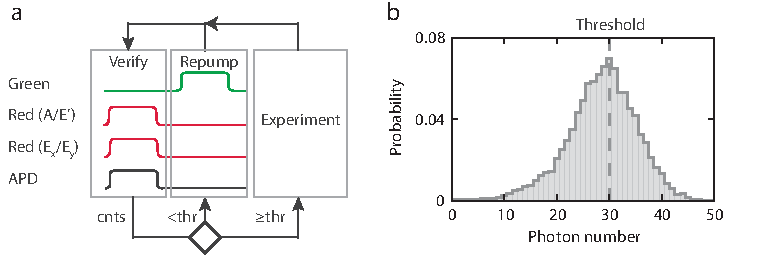
\includegraphics{CR}
	\caption{\label{fig:tam-fig4-cr} \textbf{Verifying the charge state and laser resonances} (a) Schematic of the experimental sequence to verify the charge state of the NV center and the laser resonances. The process is controlled by an ADwin microprocessor which turns on the two red lasers and compares the number of photons detected by the avalanche photodiode (APD) to a predetermined threshold (verify stage). When the number of detected photons is below the threshold a green laser is applied to prepare the $NV^-$ state (repump stage), otherwise the experimental sequence is initiated. (b) Photon number distribution during the verification stage, conditioned on the previous CR check being successful. }
\end{figure*}

The electron spin is initialized by selectively exciting a single transition\cite{Robledo_Nature_2011}: $E_x$ or $E_y$ to prepare $m_s = \pm 1$ or $A_1$/$A_2$/$E'$ to prepare $m_s=0$. The slight spin mixing of the excited states provides an optical pumping mechanism to prepare the opposite spin state (\ref{fig:tam-fig5-SP})a). The fluorescence observed during initialization (\ref{fig:tam-fig5-SP})b) exponentially decreases with the probability that the spin has flipped to a dark state that can not be excited by the pumping laser. The signal is fitted to an exponential decay to extract a lower bound for the preparation fidelity. To ensure that a pure state is prepared (as opposed to a mixture of $m_s = \pm 1$) the electron spin is typically initialized in $m_s = 0$, for this state we find a lower bound of $(99.7 \pm 0.1) \%$.

\begin{figure*}
	\centering
	\includegraphics{figure_spinpumping-bernien}
	\caption{\label{fig:tam-fig5-SP} Figure from \cite{Bernien__2014} \textbf{Initialization by spin pumping} (a) Energy levels used to initialize (and readout) the electron spin. We excite transitions with a well-defined spin character of either $m_s = 0$ (bright arrows) or $m_s= \pm 1$ (dark arrows), resulting in spin-conserving optical cycling (indicated by bended solid arrows). Dashed arrows indicate the spin non-conserving decay paths. (b) Observed fluorescence when exciting $E_x$ ($A_1$) with the spin initially prepared in $m_s = \pm 1$ ($m_s = 0$). The signal is fitted to a single exponential with an offset to account for dark counts. From the fit we find a lower limit for the initialization fidelities: $(99.7 \pm 0.1) \%$ for $m_s = 0$ and $(99.2 \pm 0.1) \%$ for $m_s=\pm 1$.}
\end{figure*}

The observed fluorescence upon selective excitation provides a means to detect the electron spin state in a single shot\cite{Robledo_Nature_2011}. To characterize the readout we plot the distribution of photons detected in the PSB collected during a 10 $\mu s$ laser pulse exciting $E_x$ (fig \ref{fig:tam-fig6-ssro}a). The distributions are clearly separated depending on the initial spin state, allowing us to assign $m_s = 0$ to the cases where one or more photons are detected and $m_s = \pm 1$ otherwise. The combined readout and initialization fidelity for $m_s = \pm 1$ ($F_1 = .989 \pm .001$) is reduced by detector dark counts and off-resonant excitation, while for $m_s = 0$ ($F_1 = .956 \pm .003$) the error is governed by the instances where the spin is flipped before a photon is detected. This can be seen in fig \ref{fig:tam-fig6-ssro}b where the readout fidelities are plotted as a function of readout duration. The fidelity for $m_s = 0$ initially increases with readout time and then saturates indicating that the spin has flipped with high probability. The optimal mean readout fidelity ($F_{ro} = \frac{F_0+F_1}{2} = 0.973 \pm 0.002$) is reached after $10 \mu s$.

\begin{figure*}
	\centering
	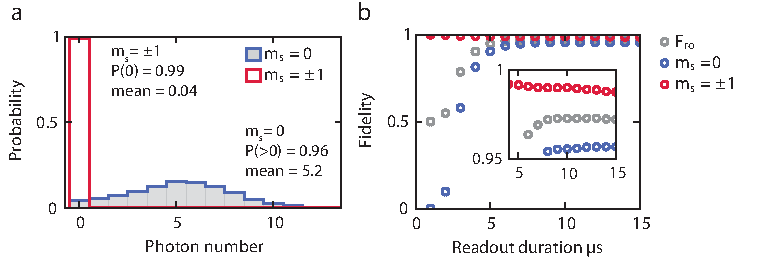
\includegraphics{ssro}
	\caption{\label{fig:tam-fig6-ssro} \textbf{Single shot readout} (a) Histograms of the number of detected photons in the PSB for initial state $m_s = 0$ (blue) and $m_s=\pm 1$ (red) during a 10 $\mu s$ readout on $E_x$. (b) Fidelities for reading out the electron spin state initially prepared in $m_s = 0$ (blue) and $m_s = \pm 1$ (red) as a function of readout duration. The mean readout fidelity is plotted in grey. The inset is a zoom of the region where the optimal mean readout fidelity is reached.}
\end{figure*}

\section{Ground state spin control}

In the orbital ground state, the $m_s = 0$ and $m_s = \pm 1$ states are separated by the zero-field splitting $D \approx 2.88$ GHz, while an external magnetic field lifts the degeneracy between $m_s = +1$ and $-1$ via the zeeman splitting. The Hamiltonian is given by

\begin{equation}
H_{GS,e} = D S_z^2 + \gamma_e \mathbf{B} \cdot \mathbf{S}
\end{equation}

with $\mathbf{S} =[S_x,S_y,S_z]$,  $S_i$ the spin matrices for a spin-1 system and $\gamma_e = 2.8$ MHz/G the gyromagnetic ratio of the electron. We define our qubit in the $m_s = 0 :\ket{0}$ and $m_s = -1 : \ket{1}$ states (alternatively the $m_s = + 1$ state can be used to encode $\ket{1}$). The electron spin is manipulated with electron spin resonance techniques by sending an ac current through the stripline generating an oscillating magnetic field at the location of the NV center. At the resonance condition the frequency of the control field matches the energy difference between the $\ket{0}$ and $\ket{1}$ states resulting in coherent Rabi oscillations between those levels as shown in fig \ref{fig:tam-fig7-erabi}. Arbitrary qubit rotations are implemented by calibrating the amplitude (which sets the rabi frequency) and length of the microwave (MW) control pulses.

\label{sec:groundstatecontrol}
\begin{figure*}
	\centering
	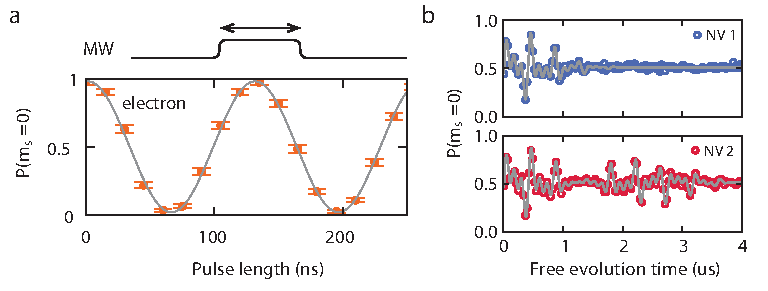
\includegraphics{electron_rabi}
	\caption{\label{fig:tam-fig7-erabi} \textbf{} (a) Coherent qubit rotations of the electron spin are performed by varying the length of a MW pulse. Solid line is a sinusoidal fit from which we determine the Rabi frequency $(7.67 \pm 0.02)$ MHz. (b) Ramsey measurements for two different NV centers where the wait time between two $\pi$/2 pulses is varied. From a fit to equation \ref{eq:tam-ramsey} we find $T_2^{*} = (0.96 \pm 0.03)$ and $(3.09 \pm 0.05) \mu$s for the upper and lower panel respectively. The coupling to the nitrogen spin is $A_{\parallel} = (2.20 \pm 0.01)$ and $(2.195 \pm 0.002) $MHz. For the bottom panel two additional frequency components are included in the fit to account for the strongly coupled $^{13}C$. We find a coupling strength of ($384 \pm 3$) kHz.  All datapoints are corrected to account for imperfect readout and initialization.}
\end{figure*}



\section{Electron spin coherence times}
\label{sec:elcohtimes}
The NV center has a long-lived electron spin state. At low temperature $T_1$-relaxation times (typical time of an eigenstate to be perturbed) were measured to be > 100 s in ensembles\cite{Jarmola_Phys.Rev.Lett._2012}. The phase coherence times depend strongly on the microscopic environment of the NV center. When the defect is located in bulk diamond (far away from any surface) the dominant dephasing mechanism is the spin-bath of the diamond lattice itself. The devices studied in this thesis are prepared from high-purity IIa CVD diamond, where the spin bath consists of $^{13}C$ isotopes (natural abundance of 1.1 $\%$). These spins create a fluctuating magnetic field at the location of the NV center that can be described by a Gaussian probability distribution with variance $b^2$. This fluctuating field changes the energy level splitting of the electron spin via the Zeeman splitting leading to dephasing on a timescale $T_2^{*} = \sqrt{2}/b$. This effect is measured in a Ramsey interferometry experiment where the accumulated phase during a free evolution $\tau$ of a superposition state is monitored (\ref{fig:tam-fig7-erabi}b). The signal is fitted with a function

\begin{equation}\label{eq:tam-ramsey}
P = A \exp(-(\tau/T_2^*)^2)\sum\limits_{k=-1}^1 \cos(2 \pi(\delta f +k A_{\parallel})\tau +\phi_k),
\end{equation}

where $\delta f$ is a detuning of the rotating frame of the microwave pulses with respect to the center frequency of the electron spin. The three frequencies arise from the coupling to the host nitrogen spin which caries a spin $I = 1$. For the NV center in the bottom panel two additional frequencies are included in the fit. They are associated with the coupling to a single $^{13}C$ spin (with spin I = 1/2), which is closer to the defect than the other spins in the bath. In this case the coupling strength of the individual $^{13}C$ spin to the electron spin is strong ($384 \pm 3$ kHz) compared to the dephasing rate $1/T_2^*$ induced by the spin bath and can therefore be individually resolved. From the gaussian decay of the fit we find $T_2^{*} = (0.96 \pm 0.03)$ and $(3.09 \pm 0.05) \mu$s for the two NV centers. The coherence times can be extended by using isotopically purified samples as shown in chapter \ref{ch:AMM} of this thesis. 

Alternatively the electron spin can be made insensitive to the static component of the fluctuating spin bath by dynamical decoupling (DD) techniques \cite{Lange_Science_2010,Ryan_Phys.Rev.Lett._2010}. Here the spin is periodically inverted by equally spaced $\pi$ pulses as shown in figure \ref{fig:tam-fig9-DD}. For a spin echo ($N = 1$) the single $\pi$ pulse inverts the direction of the accumulated phase which leads to perfect refocusing if the effective magnetic field is constant on a timescale of 2$\tau$. By increasing the number of refocusing pulses we demonstrate a coherence time ($T_{coh}$) of ($14.3 \pm 0.3$) ms for $N = 64$.

So far we presented the Ramsey and dynamical decoupling techniques as a means to characterize the coherence times of the electron spin qubit. Alternatively, one can use the observed decoherence to learn something about the microscopic environment of the NV center. Because the NV center is an atomic defect it can sense DC (Ramsey interferometry) and AC (dynamical decoupling) signals very high spatial resolution. In chapter \ref{ch:AMM} we present an experiment where real-time feedback techniques are implemented to improve the performance of such a single-spin sensor in Ramsey interferometry. As an example, the data in figure \ref{fig:tam-fig7-erabi}b demonstrates the detection of single nuclear spins near the NV center.

\begin{figure*}
	\centering
	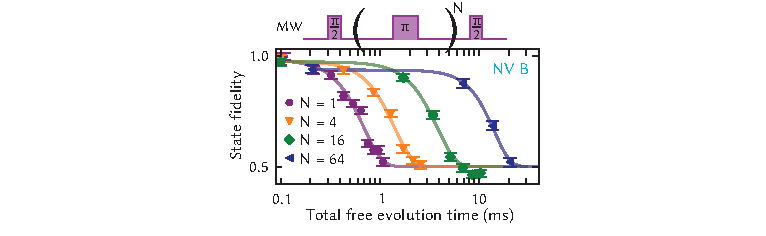
\includegraphics{DD-LDE_bernien}
	\caption{\label{fig:tam-fig9-DD} \textbf{Dynamical Decoupling of the electron spin} The coherence of the electron spin as a function of the total free evolution time $t_{FE} = 2 \tau N$ during an $N$-pulse dynamical decoupling sequence\cite{Lange_Science_2010}. The solid lines are a fit to the function $A e^{(-\frac{t{FE}}{T_{coh}})^3} + 0.5$. For $N = 64$ we find $T_{coh} = $($14.3 \pm 0.3$) ms. }
\end{figure*}

\section{Coupling to individual nuclear spins}
Nuclear spins in the vicinity of the NV center can be used to define qubits, extending the capabilities of the NV center to a multi-qubit spin register. In recent years full control of both the host nitrogen spin \cite{Gaebel_NatPhys_2006,Hanson_Phys.Rev.Lett._2006,Neumann_Science_2010,Fuchs_NatPhys_2011,vanderSar_Nature_2012} and nearby $^{13}C$ spins \cite{Jelezko_Phys.Rev.Lett._2004,Dutt_Science_2007,Neumann_Science_2008,Jiang_Science_2009,Smeltzer_Phys.Rev.A_2009,Taminiau_Phys.Rev.Lett._2012} has been demonstrated. Since the gyromagnetic ratio of nuclear spins is typically three orders of magnitude smaller compared to the electron spin, they are less sensitive to magnetic fluctuations and therefore exhibit extremely long coherence times \cite{Maurer_Science_2012}, making them very suitable quantum memories.

\subsection{Host nitrogen spin}
All NV centers have an intrinsic nuclear spin associated with the Nitrogen atom of the defect. Here we will discuss the most common isotope, used in all experiments in this thesis, namely $^{14}N$ (99.3 $\%$ abundance) which carries a spin $I = 1$. The combined electron-nuclear spin system is described by the following Hamiltonian:

\begin{equation}
H_{e,N} = H_{GS,e} - Q I_{N_z}^2 + \gamma_N \mathbf{B} \cdot \mathbf{I_N} - A_{\parallel} S_z I_{N_z} - A_{\perp}(S_x I_{N_x}+S_y I_{N_y}),
\end{equation}

with $I_{N_i}$ the Nitrogen spin matrices, $\gamma_N = 0.3077$ kHz/G the gyromagnetic ratio of the Nitrogen spin, $Q = 4.98$ MHz the quadrupole splitting and the hyperfine parameters $A_{\parallel} = 2.19$ MHz and $A_{\perp} \approx 2.1$ MHz. The experiments reported in this thesis are performed at magnetic fields where the separation between electron spin levels is large compared to the energy scale of the flip-flop terms ($S_x I_{N_x}$ and $S_y I_{N_y}$). We therefore take the secular approximation which neglect these terms such that the Hamiltonian becomes

\begin{equation}
H_{e,N} = H_{GS,e} - Q I_{N_z}^2 + \gamma_N \mathbf{B} \cdot \mathbf{I_N} - A_{\parallel} S_z I_{N_z}.
\end{equation}

For a magnetic field aligned along the z-axis of the defect, the quantization axis of the nitrogen spin is aligned with the electron spin. The parallel component of the hyperfine interaction introduces a splitting of the electron spin transitions that can be observed in a pulsed ESR measurement (figure \ref{fig:tam-fig10-nrabi}a). The three resonances correspond to the nuclear spin eigenstates labeled $m_I = +1, 0, -1$. To encode a qubit we define the logical states as $\ket{0}_N = m_i = -1$ and $\ket{1}_N = m_i = 0$ which can be manipulated with magnetic resonance techniques analogous to the electron spin manipulation (fig \ref{fig:tam-fig10-nrabi}b). The timescale of the manipulation scales inversely with the gyromagnetic ratio, resulting in a rabi frequency of ($17.07 \pm 0.01$) kHz. The nitrogen spin state is initialized and read out by mapping it to the electron spin and subsequently performing optical readout of the electron spin.

\begin{figure*}
	\centering
	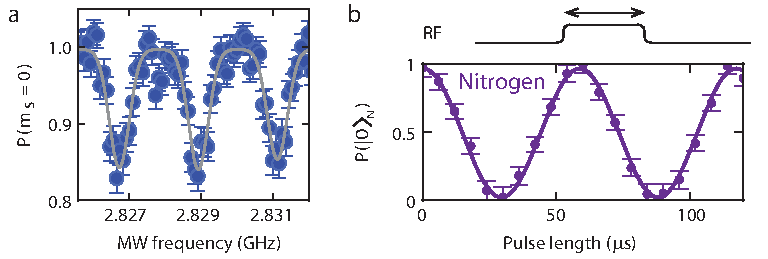
\includegraphics{nitrogen_rabi_2}
	\caption{\label{fig:tam-fig10-nrabi} \textbf{} (a) Pulsed electron spin resonance measurement of the electron spin $m_s = 0$ to $m_s = -1$ transition. The three resonances arise from the hyperfine interaction with the nitrogen spin. (b)) Coherent qubit rotations of the nitrogen spin are performed by varying the length of an RF pulse. Solid line is a sinusoidal fit from which we determine the Rabi frequency ($17.07 \pm 0.01$) kHz.}
\end{figure*}

\subsection{$^{13}C$ spins}
In addition to the nitrogen nuclear spin, each NV center is surrounded by a unique configuration of $^{13}$C-spins (with spin $I_C = 1/2$) that randomly occupy sites in the spin-free $^{12}$C diamond lattice. Again taking the secular approximation, the combined Hamiltonian for a single $^{13}$C-spin coupling to the NV center is given by:
\begin{equation}
H_{e,N,C} = H_{e,N} + \gamma_C \mathbf{B} \cdot \mathbf{I_C} + A_{\parallel,C} S_z I_{C_z} + A_{\perp,C} S_z I_{C_x},
\end{equation}

with $I_{C_i}$ the Pauli spin matrices for the Carbon spin, $\gamma_C = 1.0705$ kHz/G the gyromagnetic ratio of the Carbon spin and the hyperfine parameters $A_{\parallel,C}$ and $A_{\perp,C}$ that depend on the distance between the Carbon spin and the electron spin and on the angle with respect to the quantization axis of the NV center. Carbon spins with high coupling strength compared to the dephasing time of the electron spin ($A_C > 1/T_2^*$) can be spectrally resolved via the electron spin and allow for similar control techniques as used for the nitrogen spin \cite{Jelezko_Phys.Rev.Lett._2004,Dutt_Science_2007,Neumann_Science_2008,Jiang_Science_2009,Smeltzer_Phys.Rev.A_2009}. A signature of a strongly coupled carbon spin can be seen in figure \ref{fig:tam-fig7-erabi}b (bottom panel). Recently it was shown that dynamical decoupling techniques can overcome the limitation set by the electron spin decoherence to detect\cite{Taminiau_Phys.Rev.Lett._2012,Kolkowitz_Phys.Rev.Lett._2012,Zhao_NatNano_2012} and control\cite{Taminiau_NatNano_2014} weakly coupled Carbon spins. In chapter \ref{ch:CDL} and \ref{ch:CDP} we investigate the feasibility to use these weakly coupled carbon spins as quantum memories that are robust against optical excitation of the electron spin.

\section{Initialization by Quantum measurement}
The nuclear spins (nitrogen or carbon) can be prepared via measurement-based initialization\cite{Robledo_Nature_2011}. According to Born's rule a projective measurement associated with operator $\hat{A}$ of a system initially in a state $\ket{\psi_S}$ collapses the system to one of the eigenstates $\ket{\lambda_i}$ of $\hat{A}$ with probability $p_i = |\braket{\lambda_i}{\psi_S}|^2$. When the system is initially in an unknown state described by the density matrix $\rho_S$ the post-measurement density matrix, given measurement outcome $\lambda_i$ is

\begin{equation}
\rho_{S|\lambda_i} = \frac{1}{p_i}\hat{P}\rho_S\hat{P}
\end{equation}

with $\hat{P}=\ket{\lambda_i}\bra{\lambda_i}$, leaving the system in a pure state even if the initial density matrix is mixed. For the nitrogen spin the qubit states are eigenstates of the operator $I_{N_z}$. Thus to initialize it we perform a measurement of this operator and continue with the experiment when the measurement result corresponds to the desired state.

We perform a measurement of $I_{N_z}$ of the nitrogen spin by implementing an indirect von Neumann measurement using the electron spin (Fig. \ref{fig:tam-fig11-mbi}). In this scheme the system (nitrogen spin) is first mapped onto a probe (electron spin) with an entangling operation. As a result the information about the system is encoded in the probe which is then measured. In our case the electron is initially prepared in $m_s= \pm 1$ and then flipped with a microwave pulse that is conditional on an eigenstate of the nitrogen. When the subsequent electron spin readout yields $m_s = 0$, the nitrogen spin is projected to the corresponding eigenstate as verified by electron spin resonance (Fig. \ref{fig:tam-fig11-mbi}).

\begin{figure*}
	\centering
	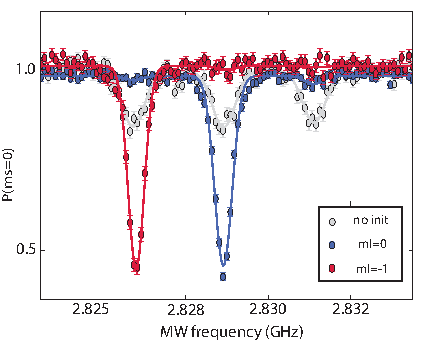
\includegraphics{MBI}
	\caption{\label{fig:tam-fig11-mbi} \textbf{Measurement-based initialization of the nitrogen spin}. Pulsed electron spin resonance for no initialization of the nitrogen spin (grey) and after performing measurement-based initialization of the nitrogen spin in $m_I = -1$ (red) and $m_I = 0$. The polarization of the nitrogen spin is inferred from the depth of the observed resonances.}
\end{figure*}

For measurement-based protocols like initialization by measurement and quantum error correction\cite{Devoret_Science_2013} it is crucial that the measurement is quantum non-demolition (QND)\cite{Braginsky_Science_1980}, meaning that the final state of the system is exactly the eigenstate associated with the measurement outcome such that two consecutive measurements of the same observable yield the same result. In practice this is not always the case since a measurement could completely destroy the system (as is the case for measuring a photon with an APD) or the measurement process itself can introduce additional disturbance. An example is the optical readout of the electron spin where a finite spin-flip probability in the excited state can leave the electron spin in a dark state regardless of the measurement outcome.In chapter \ref{ch:AMC} we introduce a QND measurement of the electron spin and use it to implement a partial measurement of the nitrogen spin and study the measurement backaction. In chapter \ref{ch:LDE} of this thesis we use a projective measurement to prepare two remote qubits in an entangled state.

\newpage
\bibliographystyle{../thesis}
\bibliography{tam}


